%\begin{flushright}
%%%\emph{``For the things we have to learn before we can do them, we learn by doing them.''}\\%Each wrong scenario you have analysed, is a wrong decision you won't made.''}\\
%%%Aristote
%\emph{All models are wrong, but some are useful.}\\
%George P. Box
%\end{flushright}

%\medskip
%
%\begin{mybox}{Chapter overview}
%\begin{itemize}[left=0em]%[leftmargin=0cm,itemindent=.5cm,labelwidth=\itemindent,labelsep=0cm,align=left]
%\setlength\itemsep{-0.3em}
%\item Belgian energy system overview%Case studies: the Belgian energy systems during the transition (2015-2050).
%\end{itemize}
%\vspace{-0.3cm}
%
%\emph{This chapter is an improved and extended case study version of \citet{Limpens_belgian_2020}}.
%\end{mybox}
%
%\medskip

As detailed by \citet{limpens2024pathway}, the analysis carried out in this work can be applied to any regional whole-energy system. As a densely-populated and highly-industrialised country with limited local renewable potentials (\ie mainly solar and wind representing up to 50\% of the primary mix by 2050), the transition of Belgium from a fossil-dominated system in 2020 (Appendix \ref{app:bel_2020}) to carbon-neutrality in 2050 makes it an intricate case study. Moreover, this case study and the subsequent analyses can be transferred - to some extent - to other industrialised countries highly dependent on fossil fuels with limited local renewable potentials (\eg the Netherlands or Germany) \cite{dommisse2020modelling}. This chapter presents the different demands to satisfy, with a particular focus on the non-energy demand, as well as the resources available and the conversion technologies to supply those. For a comprehensive understanding and detailed descriptions of the technologies, please refer to the documentation \cite{readthedocs_pathway}. Then, the uncertainty ranges considered for some of the parameters are detailed. Finally, the \ce{CO2}-budget over the 2020-2050 transition is presented.

\section*{Contributions}
\label{sec:cs:contributions}
First, as pointed out by \citet{rixhon2022integration}, where most of the studies assessing whole-energy system integrate energy demands (\ie electricity, heart and mobility), the \acrfull{NED} is often not considered. The latter is defined as ‘\textit{energy products used as raw materials in the different sectors; that is not consumed as a fuel or transformed into another fuel}’ \cite{Eurostat2019}. The previous analyses carried out with \gls{ESTD} considered the non-energy demand as the related primary energy needs, \ie either natural gas or \gls{LFO}. To minimise the total cost of the system, the model simply selected the cheapest between the two resources (\ie natural gas). This work goes one step further and accounts for the \gls{NED} as a demand of three commodities (\ie \gls{HVC}, ammonia and methanol) as well as with associated production technologies. This allows bringing the non-energy sector to a similar level of details as the other sectors.  Keeping the same methodology to define \gls{EUD} in EnergyScope as \citet{Limpens2020}, this work considers updated values given the latest release of the \og EU reference scenario 2020 : energy, transport and GHG emissions: Trends to 2050 \fg by the European Commission \cite{EuropeanCommission2021}.

Second, given the focus of this work on the electrofuels, the case study includes a more explicit representation of them: where the previous definition of the case study considered only renewable hydrogen and methane \cite{limpens2021generating}, now, e-ammonia and e-methanol (as well as their fossil-based equivalents), are implemented in the case study. As detailed later on, these electrofuels are considered as renewable in the sense that their \gls{GWP} is zero. This more explicit representation of the molecules themselves also comes with a more exhaustive integration of the ways to produce and use them in the system. For instance, considering the case of ammonia, on the top of the import routes, the Haber-Bosch process ,on one hand, is accounted for to supply this molecule. On the other hand, ammonia-driven \gls{CCGT} or ammonia-cracking-to-hydrogen are included as ways to consume it.

Third, as nuclear energy could be a real game-changer in the energy transition worldwide \cite{IEA2022nuclear}, and especially in Belgium, this thesis has integrated the uncertain potential to install \gls{SMR} from 2040 onward.

Fourth, where previous works considered a prescribed \ce{CO2} trajectory to reach carbon-neutrality by 2050 \cite{limpens2021generating, limpens2024pathway}, the case study analysed in this thesis is subject to a \ce{CO2}-budget for the transition, \ie limiting the total amount of emissions over the transition. Based on the estimated world budget provided by the \gls{IPCC} to limit the global warming to +1.5°C by the end of the century, the grandfathering approach has been used to allocate part of this budget to the Belgian energy transition.

Finally, to a smaller extent, this work includes updated values for some parameters compared to the work of \citet{limpens2021generating}. The main change concerns the cost and performance of private mobility vehicles, which is specifically a key components in the European \cite{biresselioglu2018electric} and Belgian \cite{BFP_mob} energy transitions. Based on the work of \citet{national2013transitions}, \citet{limpens2021generating} excessively favoured \gls{FC} car versus \gls{BEV}. Besides their lower efficiencies (\ie about 50\% less efficient), \gls{FC} car had the lion share of the private mobility, compared to \gls{BEV} given the higher CAPEX (\ie up to 10\% more expensive) and limited range (\ie 24kWh battery) of the latter, in previous works \cite{limpens2021generating,rixhon2021role}. In these, the more limited potential to import electricity from abroad and produce it locally via \gls{VRES} forced the model to rather electrify the low-temperature heat sector rather than the private mobility running on supposedly infinitely available renewable hydrogen. To align with other similar works on the modelling of whole-energy system \cite{schnidrig2021modelling, EuropeanCommission2021}, the CAPEX and efficiency of fuel cell cars have been increased. Regarding \gls{BEV}, while the CAPEX has been kept unchanged, the efficiency and the battery capacity, \ie the range, have been increased. As seen in the results, this change of data made \gls{BEV} often more competitive than its hydrogen-based equivalent. 

\section{End-use demands}
\label{sec:cs:demand}
End-use demands, exogenously imposed as inputs to the model, are characterised by yearly quantities to satisfy and are also distributed over the different hours of each representative years of the transition, in order to account for their daily or seasonal variability \cite{Limpens2020,limpens2021generating}. In this work, the yearly end-use demands (EUD) for all sectors are calculated from the forecast proposed by the European Commission for Belgium (Appendix 2 in report \cite{EuropeanCommission2021}). 

\subsection{Non-energy demand}
\label{subsec:cs:NED}
The \gls{NED} currently represents around 20\% of the final energy consumption in Belgium \cite{FPSEconomy2021}.  This section summarises the rationale of adding a higher level of details to the\gls{NED} compared to what was done in the previous version of the case study \cite{limpens2021generating}. Then, it explains the methodology used to quantify this demand.\\

\myparagraph{Definition and historical trend}\\

\noindent
The \gls{NED} can be split into four main categories of final molecules \cite{IEA2018_petrochemicals}: (i) \gls{HVC} (worldwide production of $\sim$365Mt/year, equivalent to $\sim$4770TWh/year); (ii) ammonia ($\sim$185Mt/year, equivalent to $\sim$964TWh/year); (iii) methanol ($\sim$100Mt/year, equivalent to $\sim$540TWh/year) and (iv) the other products. \Gls{HVC} gather the light olefins (e.g. ethylene, propylene) and aromatics (benzene, toluene, xylene – BTX), mainly for the production of plastics, synthetic fibers or rubber. Their production today relies mainly on petroleum products such as naphtha, ethane or liquified petroleum gas. Ammonia is  mainly used for the production of fertilizers ($\sim$80\% of global ammonia consumption). Its production is dominated by fossil gas via steam methane reforming to produce hydrogen, used as feedstock in the Haber-Bosch process. Methanol is mainly converted to formaldehyde (resin) but also used for the production of other chemicals (e.g. solvents and gasoline-blends). Currently, its synthesis, like ammonia, is mainly relying on natural gas via steam methane reforming. Finally, the other products gather all chemicals not mentioned in the other categories such as bitumen, lubricants and other heavy products from oil refineries \cite{daioglou2014energy}.

Over the recent history, there has been a relatively constant evolution of three main categories of the final consumption for non-energy use in Belgium, \cite{statbel_NED_2019}: (i) naphtha and \gls{LPG} (between 59\% and 67\% of the total final consumption, around 59.4\,TWh in 2019), (ii) fossil gas (between 9\% and 14\%, 11.8\,TWh in 2019), and (iii) others (\ie bitumen, coal tar and other oil products) (between 21\% and 28\%). Naphtha and \gls{LPG} are consumed in a naphtha cracker, which results in ethylene and propylene, what will be considered as \gls{HVC} in the rest of this work. Similarly, fossil gas, as non-energy carrier, is used in steam methane reformer to produce the required hydrogen to the synthesis process of ammonia. The small shares of bitumen and coal tar are respectively used for roadworks and to produce synthetic gas through gasification. Finally \og other oil products'' take into account, indistinguishably, tar and sulphur as well as by-products of the refineries (\eg \gls{BTX}). About methanol, there is currently no production plant in Belgium even if the country plays a role in trading this commodity between its neighbouring countries and consumes part of what it imports.\\

\myparagraph{Methodology of quantification}\\

\noindent
The non-energy demand studied in this analysis focuses on the chemical industry (more than 90\% of the non-energy use in Belgium) and, similarly to other studies \cite{IEA2018_petrochemicals, daioglou2014energy}, is split between the three aforementioned main groups of products (\ie \gls{HVC}, ammonia and methanol). Before describing these three demands, this study excludes bitumen, coal tar and \og other oil products\fg. The first two represent marginal shares of the current non-energy use (\ie 4\% and 5\% respectively) in such a way that they should not affect the conclusions provided by this study. As described previously, the latest are mostly by-products from refineries that the system uses because they are available. However, in a perspective of defossilisation, since the future of fossil-based refineries is unclear, they have not been implemented in this study nor their by-products.

Regarding \gls{HVC}, the future of their production is highly uncertain. Because of the new regulations and strategies promoting recycling and limitation of single-use plastics \cite{EU_plastics}.  Besides this uncertainty, Belgium stays a major exporter as approximately 2/3 of plastic raw materials produced locally are exported abroad \cite{agoria_plastics}. Even if a significant part of \gls{HVC} produced in Belgium is not locally consumed, this demand has been set based on the assumption that Belgium will keep its industrial activity in this sector. In other words, this assumption does not deduce the part of local production  of \gls{HVC} being then exported (and not consumed locally), unlike ammonia and methanol, which will be more traded commodities in the future (as energy carriers and non-energy products). Therefore, the actual demand of \gls{HVC} is inferred from the consumption of naphtha and \gls{LPG} as non-energy use as well as energy-carrier in the chemical and petrochemical industries \cite{statbel_NED_2019}. This assumption is based on the fact that, in the conversion processes to produce \gls{HVC} from naphtha or \gls{LPG}, these fuels also serve as energy-carrier to supply the process itself. Then, given the respective efficiencies (1.83t$_{\text{naphtha}}$/t$_{\text{HVC}}$ and 1.67t$_{\text{LPG}}$/t$_{\text{HVC}}$) \cite{IEA2018_petrochemicals}, the current demand of \gls{HVC} is estimated equal to 3069\,kt, without making distinctions between the different chemicals (\ie ethylene, propylene and \gls{BTX}). 

The ammonia sector in Belgium is quite different: the country locally produces and imports ammonia much more than it exports it. Thanks to a database from the United Nations \cite{UN_statistics} and the National Bank of Belgium, it has been identified that, over the last ten years, Belgium has imported 1010\,kt of ammonia, exported 105\,kt and locally produced 990\,kt on average. Therefore, on top of the local production, the net import (\ie import minus export) is also included in this non-energy demand. This gives a current demand of 1895\,kt of ammonia.

Concerning the demand of methanol, similarly to ammonia, this work solely considers the net imports as there is no local production in Belgium. To define the actual non-energy demand of methanol, only a 51\%-share of this net import is kept since, according to the Methanol Institute and \gls{MMSA}, this share is used for formaldehyde production in Belgium \cite{MMSA51}. Currently, the rest of the methanol is used for energy purposes, mostly as \gls{MTBE} in gasoline blending. This methodology gives a current non-energy demand of methanol of 269\,kt.

Eventually, after converting these masses of products into energy content (\ie LHV: \gls{HVC} - 47\,MJ/kg, ammonia - 18.8\,MJ/kg and methanol - 19.9\,MJ/kg), two final assumptions are made: (i) the current shares of each of the three commodities (\ie 77.9\%, 19.2\% and 2.9\% for \gls{HVC}, ammonia and methanol, respectively) are supposed to remain unchanged over the transition; (ii) the overall \gls{NED}, in absolute terms, follows the growing rate presented by \citet{EuropeanCommission2016}, \ie around 7\% between 2020 and 2050.

\subsection{Forecast of the demands over the transition}
\label{subsec:cs:EUD_forecast}
In their latest report \cite{EuropeanCommission2021}, the European Commission forecasts a significant and abrupt increase of the \gls{NED} compared to their previous report \cite{EuropeanCommission2016}, \ie +80\% over the 2020-2030 time window. Given this discrepancy that is unsubstantiated and specific to the case of Belgium, the evolution trend of the \gls{NED} of the current work has been inferred from the previous edition, published in 2016, \cite{EuropeanCommission2016}. Between 2020 and 2050, one observes a noteworthy increase of the electricity (+40\%), passenger (+45\%) and freight mobility (+35\%) demands (see \Cref{fig:cs_demands}). The rise of the non-energy demand is more limited, \ie +6\%, whereas the heating demands is forecast to decrease: -11\% for the low-temperature heat demand and -3\% for the high-temperature heat demand. This is explained by a better insulation of buildings and an improved efficiency of industrial processes. Regarding the center graph of \Cref{fig:cs_demands}, it is the aggregation of the same data as in the left graph but per category, rather than per sector, with the non-energy demand being associated with the industry. This illustrates how industrialised is Belgium, compared to households and services, and, consequently, highly energy-intensive. The right graph of \Cref{fig:cs_demands} gives the passenger and the freight mobility. The sharp increase from 2020 to 2025 is due the COVID-crisis that has significantly reduced these demands in 2020. As far as the hourly discretisation of these demands is concerned, time series are based on historical values of 2015 for the fluctuating parts of electricity and low-temperature heating demands \cite{Limpens2020}. A daily time series is used for the passenger mobility and applied similarly to every days of the year. Finally, for the other demands (\ie high-temperature heat, freight mobility, \gls{NED} and constant share of electricity and low-temperature heat demands), the yearly demand is distributed uniformly over the different hours of the year.

\begin{figure}[htbp!]
\centering
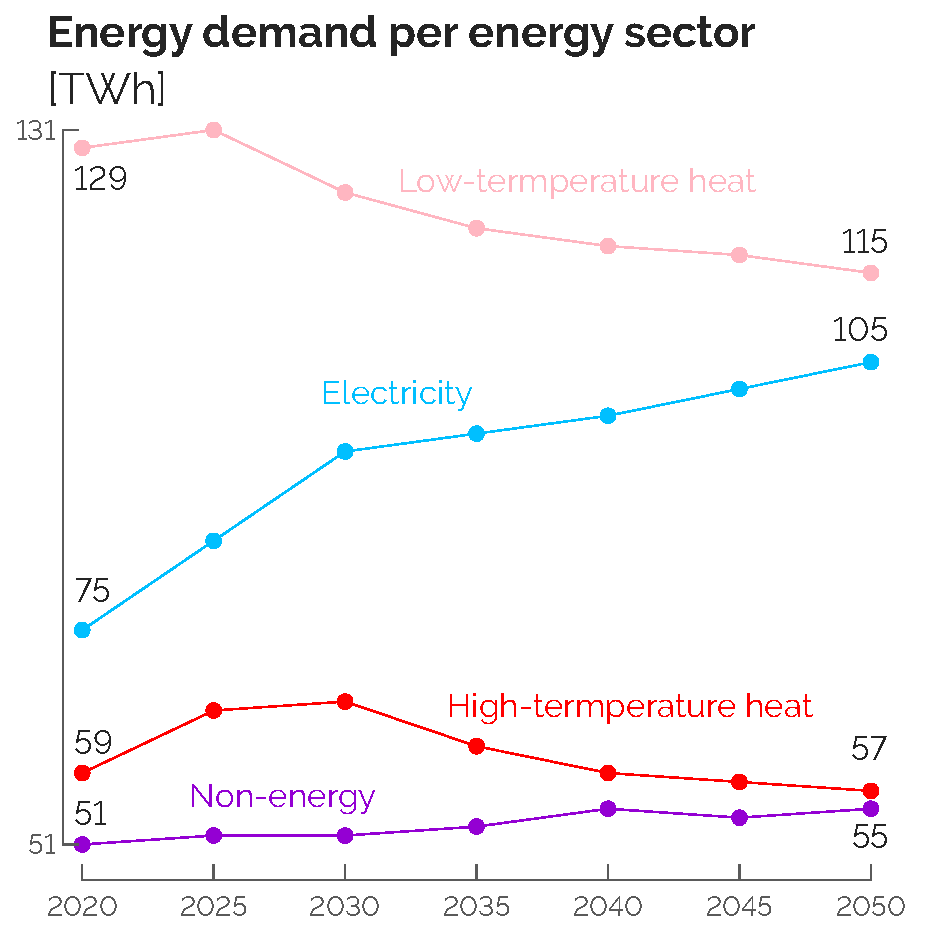
\includegraphics[width=0.49\textwidth]{EUD_sec.pdf}
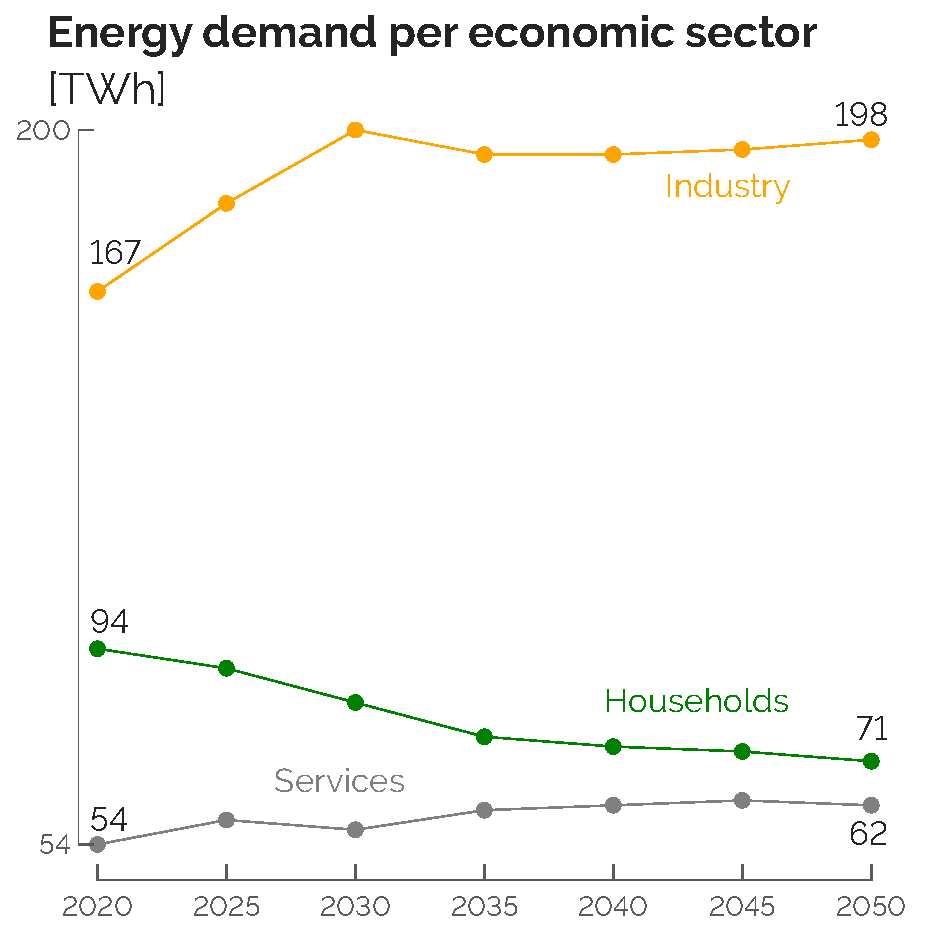
\includegraphics[width=0.49\textwidth]{EUD_cat.pdf}
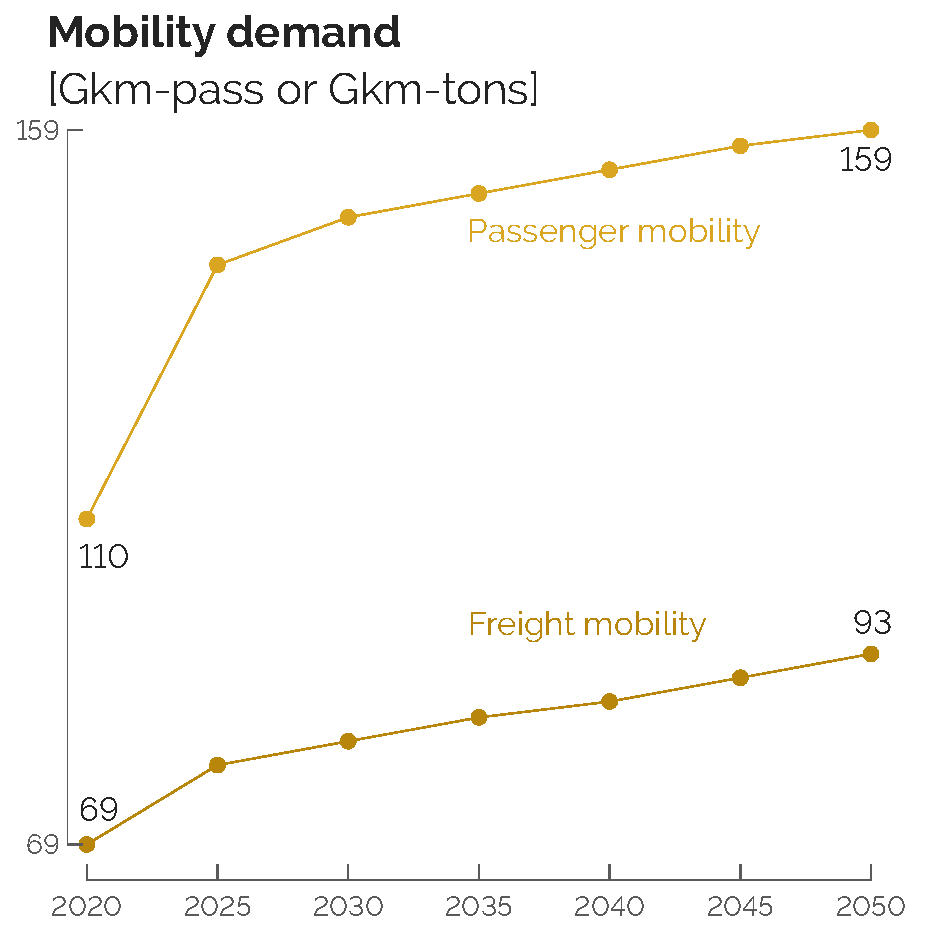
\includegraphics[width=0.49\textwidth]{EUD_mob.pdf}
\caption{EnergyScope splits the whole-energy system end-use demands (EUD) into two sets: (non)-energy and transport-related. This figure presents the nominal values of each of these demands. In the center graph, the non-energy demand has been fully associated with the industrial demand. As detailed previously, the non-energy demand is expressed in tons of physical products (\ie \glsxtrfull{HVC}, ammonia and methanol) and then translated into their respective energy equivalent, in TWh.}
\label{fig:cs_demands}
\end{figure}


\section{Resources}
\label{sec:cs:resources}
To supply the aforementioned demands, EnergyScope Pathway implements a variety of resources defined by their cost of purchasing, $\mathit{c}_{\mathrm{op}}$, their global warming potential, $\emph{gwp}_{\mathrm{op}}$, as well as their 
availability, as detailed by \citet{limpens2024pathway}. First, the evolution of the respective costs of purchasing is presented (see \Cref{fig:cs_resources_cost}). Regarding ``renewable electrofuels'', these are in line with the recent study of \citet{genge2023supply} who carried out an extensive review and ``meta-analysis\cite{grant2009typology,page2021prisma} of 30 studies on the supply costs of chemical energy carriers''. Then, besides their cost, the resources are either limited or unlimited in terms of availability and either renewable or not. The limitation in terms of availability can be direct or indirect. On the one hand, woody (23.4\,TWh) and wet biomass (38.9\,TWh) are arbitrarily limited by their local potentials and the consumption of waste (17.8\,TWh) and coal (33.4\,TWh) is assumed not to exceed the current use. On the other hand, wind, solar, hydro and uranium are limited by the technical potentials of \gls{PV} panels (59.2\,GW), onshore (10\,GW) and offshore (6\,GW) wind turbines, run-of-the-river power plants (0.1\,GW) and nuclear power plants (6\,GW), respectively. In line with the work of \citet{PATHS2050} and the maximum capacity of conventional nuclear reactors that have been installed in Belgium, the same 6\,GW are assumed to be the maximum capacity for \gls{SMR}. Imported electricity is limited in two ways: the potential of instantaneous capacity of interconnection with neighbouring countries (\ie 11.9\,GW by 2050 \cite{ELIA_2050}) and a limitation to 30\% of the yearly electricity end-use demand (\ie 32.4\,TWh by 2050) \cite{limpens2021generating}. In the current work, the electrofuels (\ie e-methane, e-hydrogen, e-methanol and e-ammonia) are assumed to be ``sustainable" in the sense that they do not increase the concentration of \ce{CO2} in the atmosphere \cite{rixhon2021terminology}. In practice, it means that their \gls{GWP} is assumed to be zero in the model. Regarding specifically these electrofuels, the \citet{h2coalition} has carried out an extensive techno-economic analysis to estimate their respective cost of purchasing, after having identified some key locations from which importing these energy carriers (\eg Chile, Australia or Morocco). As the amount to import from each of these locations is hard to forecast, the current work considers the average cost between the different locations. Besides these, every other resource has its specific \gls{GWP} like coal ($\emph{gwp}_{\mathrm{op,coal}}=0.40$\,kt$_{\ce{CO2},\text{eq}}$/GWh), natural gas ($\emph{gwp}_{\mathrm{op,NG}}=0.27$\,kt$_{\ce{CO2},\text{eq}}$/GWh) or the fossil-based molecules equivalent to the electrofuels (\eg $\emph{gwp}_{\mathrm{op,ammonia}}=0.46$\,kt$_{\ce{CO2},\text{eq}}$/GWh or $\emph{gwp}_{\mathrm{op,methanol}}=0.41$\,kt$_{\ce{CO2},\text{eq}}$/GWh).

\begin{figure}[htbp!]
\centering

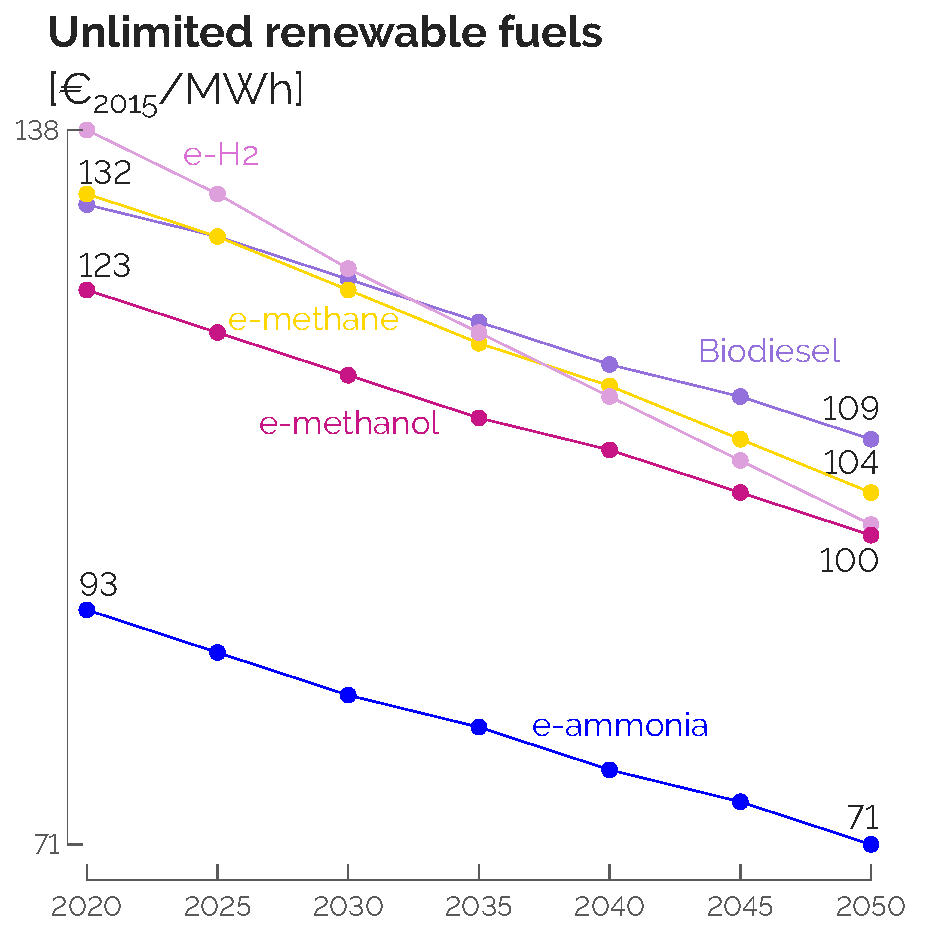
\includegraphics[width=0.49\textwidth]{Res_ren.pdf}
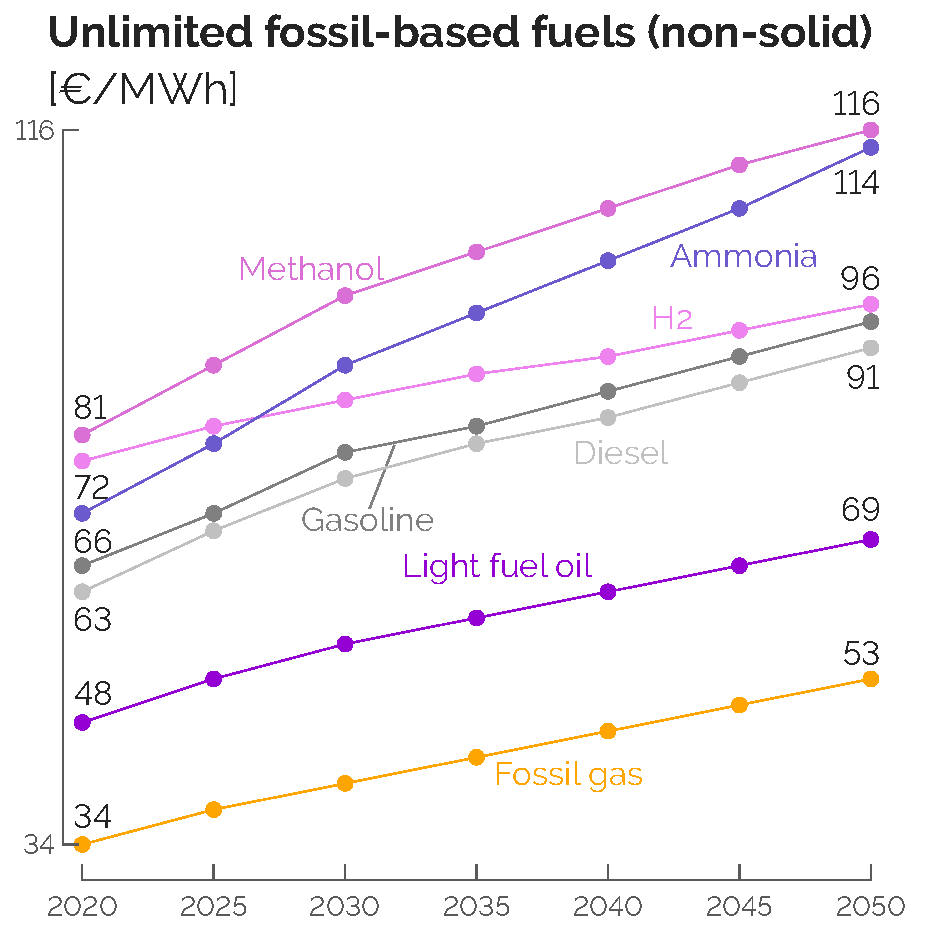
\includegraphics[width=0.49\textwidth]{Res_foss.pdf}
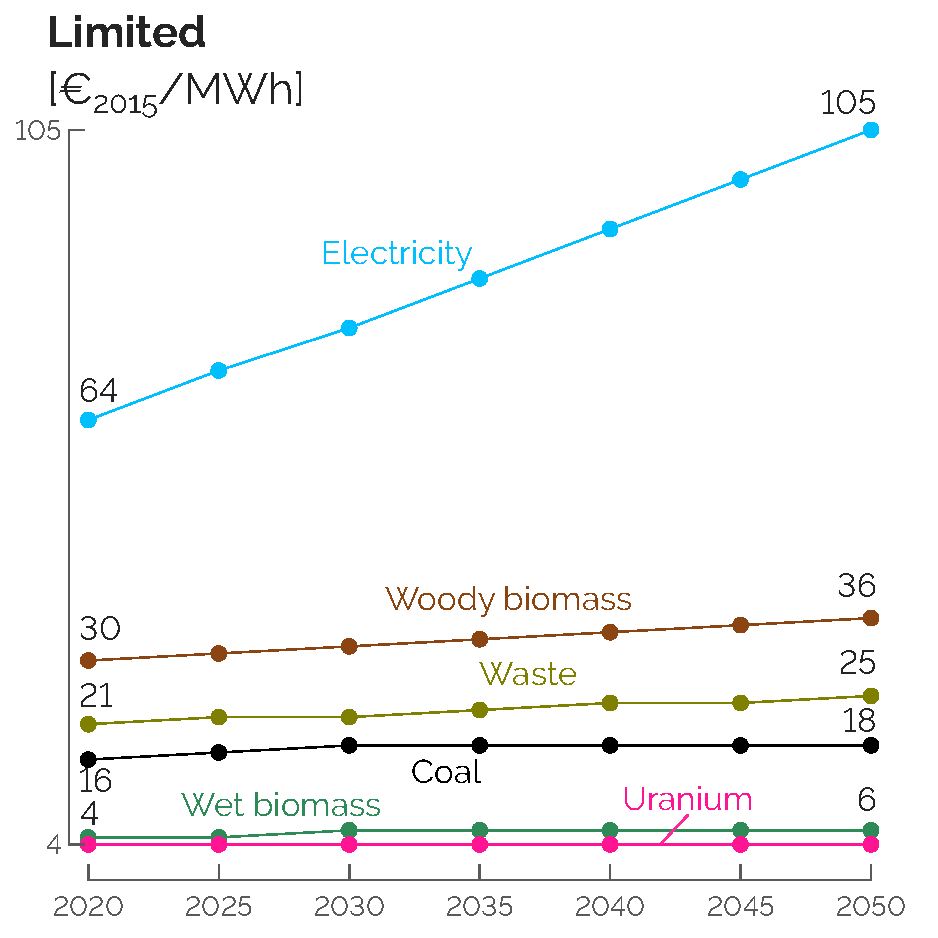
\includegraphics[width=0.49\textwidth]{Res_others.pdf}
\caption{Cost of purchasing the different resources. Besides the free local renewables (\ie sun, wind and hydro) limited by technical potentials, EnergyScope accounts for renewable energy carriers and their respective fossil counterparts (left and center graphs). These fuels can be imported from abroad without limitation on their availability. Other carriers are limited either by their local potentials (\ie biomass and waste) or other considerations like the power grid interconnections or the capacity of nuclear power plants.}
\label{fig:cs_resources_cost}
\end{figure}


\section{Conversion technologies}
\label{sec:cs:technologies}
As the end-use demands are defined as energy (and non-energy with the \gls{NED}) services rather than a certain quantity of oil or solar irradiance, for instance, technologies are implemented to convert these resources into the end-use demands. Besides their CAPEX, OPEX and lifetime defined in Section \ref{sec:meth:ES}, production and conversion technologies (\ie \gls{CCGT}, car or boiler) have a conversion efficiency whereas storage technologies (\ie thermal storage, battery or molecule storage) exhibit their own charge/discharge losses. There are also infrastructure technologies. They encompass, for instance, the power grid, the \gls{DHN} or technologies to produce intermediate energy carriers (\eg wood pyrolysis, biomethanolation or steam methane reforming to produce hydrogen). Not digging into too much details about the exhaustive list of these technologies presented in previous works \cite{limpens2021generating}, this section rather focuses on the implementation of \glsxtrfull{SMR} then the technologies to supply the \glsxtrfull{NED}.

\subsection{Small modular reactor}
\label{subsec:cs:SMR_tech}

A specific attention is to put on the implementation of \gls{SMR} whereas the 6\,GW of conventional nuclear are assumed to drop to 2\,GW in 2025 and total phase-out by 2035. Similarly to the analysis of \citet{PATHS2050}, a Belgian consortium for energy research, and in line with the Belgian Nuclear Research Centre (SCK-CEN) \cite{SCK-CEN_SMR}, \gls{SMR} are implemented with the features listed in \Cref{tab:SMR_features}. Where most of the features are similar to conventional nuclear power plants, it differs from these on two main points: their potential year start, 2040, and their flexibility. Indeed, unlike the current nuclear power plants, constrained in the model to produce a constant power output at every hour of the year (\ie baseload production as it is actually the case in Belgium), SMRs, are flexible in the sense that their production can vary between 0 and their full capacity independently at any hour of each representative year. Here, we simplify SMRs as only producing electricity and disregard the heat produced by the nuclear reaction. This is considered as lost to the atmosphere.

\begin{table}[htbp!]
\caption{Nominal features of the SMRs in EnergyScope. \gls{SMR} exhibits the advantage to have a fully flexible production (\ie between 0 to the full capacity) unlike conventional nuclear that is constrained to produce a constant baseload at every hour of the year.}
\label{tab:SMR_features}
\begin{minipage}{\linewidth}
\centering
\begin{tabular}{l c c}
\toprule
\textbf{Feature} & \textbf{Value} & \textbf{Unit}\\
\midrule
CAPEX & 4850 & €/kW \\
Annual OPEX & 103 & €/kW/year \\
Lifetime & 60 & year \\
Efficiency & 40\% & -\\
Maximum capacity & 6 & GW \\
Annual availability & 85\%\footnote{\label{foot:avail_SMR}This annual availability accounts for yearly maintenance where the reactors might not operate or, at least, not at their maximum capacity. } & -\\
Operational year & 2040\footnote{\label{foot:op_year_SMR}2040 is the soonest year at which \gls{SMR} could be available, optimistically assuming industrial prototypes being completed by 2035 and 5 additional years for their commercial installation.} & - \\
Flexibility & Full & - \\
\bottomrule							

\end{tabular}
\end{minipage}
\end{table}


%\begin{table}[htbp!]
%\caption{Nominal features of the SMRs in EnergyScope. \gls{SMR} exhibits the advantage to have a fully flexible production (\ie between 0 to the full capacity) unlike conventional nuclear that is constrained to produce a constant baseload at every hour of the year.}
%\label{tab:SMR_features}
%\centering
%\begin{tabular}{l c c|c}
%\toprule
%\multirow{2}{*}{\textbf{Feature}} & \multirow{2}{*}{\textbf{Value}} & \multirow{2}{*}{\textbf{Unit}} & \textbf{Similarity with}\\
% & & & \textbf{conventional nuclear}\\
%\midrule
%CAPEX & 4850 & €/kW & \checkmark\\
%Annual OPEX & 103 & €/kW/year & \checkmark\\
%Lifetime & 60 & year & \checkmark\\
%Efficiency & 40\% & -& \checkmark\\
%Maximum capacity & 6 & GW & \checkmark\\
%Annual availability & 85\%\footnote{\label{foot:avail_SMR}This annual availability accounts for yearly maintenance where the reactors might not operate or, at least, not at their maximum capacity. } & -& \checkmark\\
%\midrule
%Operational year & 2040\footnote{\label{foot:op_year_SMR}2040 is the soonest year at which \gls{SMR} could be available, optimistically assuming industrial prototypes being completed by 2035 and 5 additional years for their commercial installation.} & - & \xmark\\
%Flexibility & Full & - & \xmark\\
%\bottomrule							
%
%\end{tabular}
%\end{table}

For the sake of comparison, the \gls{LCOE} of the principal technologies to produce electricity, based on the computation used by \citet{limpens2021generating}, are detailed (see \Cref{fig:LCOE}). Not including here the cost of integrating a technology in the system (\eg reinforcement of the grid and storage capacities for \gls{VRES}), the \gls{LCOE} aims at aggregating and normalizing the CAPEX and OPEX of technologies providing a common commodity, \ie electricity. Compared to the other flexible generation units (\ie \gls{CCGT}), \gls{SMR} is significantly more cost-effective. Besides being about six times more capital-intensive in €/kW, the investment is amortized over a longer expected lifetime (\ie 60 years versus 25 for \gls{CCGT}). Moreover, the cost of purchasing uranium driving \gls{SMR} is expected to remain stable and low whereas the expected increase of the cost of purchasing fossil fuels dominates the \gls{LCOE} of \gls{CCGT}. In addition, one sees that \gls{CCGT} supplied by e-ammonia outcompetes its e-methane equivalent, unlike their respective fossil-based equivalent. This due to the fact that e-ammonia, not requiring carbon capture, is expected to be more cost-effective to produce versus e-methane \cite{h2coalition}. On the contrary, fossil-based ammonia, mostly relying on steam methane reforming, requires additional steps in the production process compared to fossil gas, as introduced in Section \ref{subsec:cs:NED}.

\begin{figure}[htbp!]
\centering
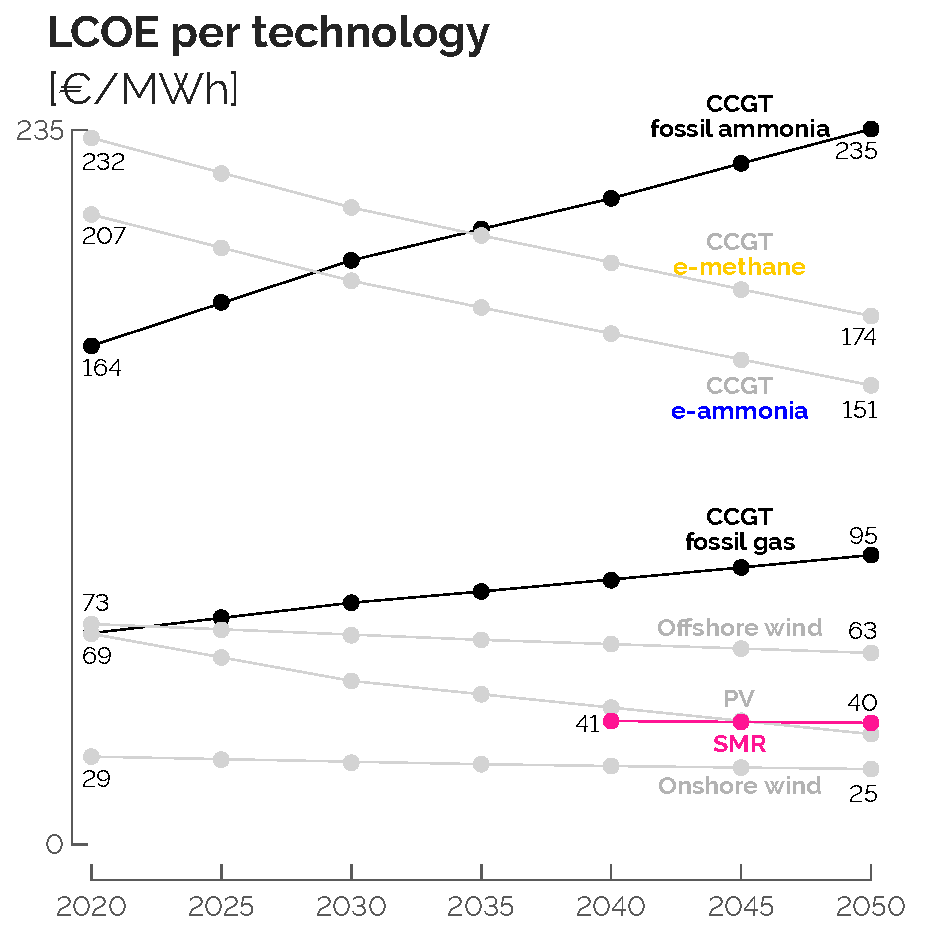
\includegraphics[width=0.49\textwidth]{LCOE_line_2.pdf}
\caption{Levelised cost of energy (LCOE) for the main technologies in the power sector. Gray and black curves are related to technologies runnning on renewable and fossil resources, respectively. Where \gls{SMR} is cheaper than the other flexible options, \gls{CCGT} running on e-ammonia is, a priori, cheaper than its e-methane alternative.}
\label{fig:LCOE}
\end{figure}

\subsection{Technologies supplying the non-energy demand}
\label{subsec:cs:NED_tech}

Different paths are implemented to produce the final molecules of the NED (see \Cref{fig:NED_tech}). Similarly to \citet{tsiropoulos2018emerging}, naphtha, here considered as \gls{LFO}, resulting from refinery operation is modeled as an imported commodity. Presented here for the specific year of 2035, all data and related references can be found in \cite{GIT_NED}. To keep the same level of details with other sectors of the model, the implementation of the conversion technologies consists of a single kind of technology per type of resource to produce a certain product. For instance, in the model, there is only one technology to produce \gls{HVC} either from naphtha or from LPG, two liquid fossil hydrocarbons, \ie \gls{NSC}. For ammonia and methanol, the molecules can either be produced locally from other resources or directly imported (with distinction between non-renewable and renewable molecules). 

\begin{figure}[htbp!]
\centering
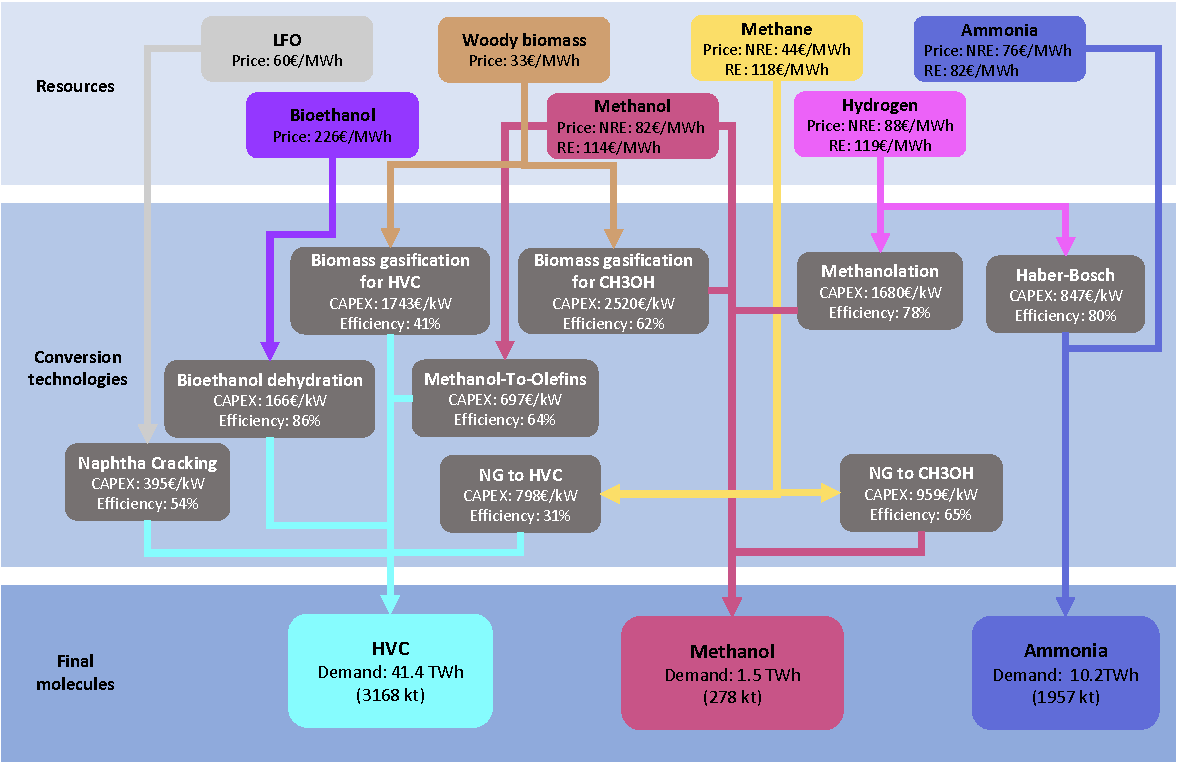
\includegraphics[width=0.8\textwidth]{NED_tech.pdf}
\caption{Schematic view of the different resources able to produce \gls{HVC}, ammonia and methanol with their related conversion technologies (including energy efficiency and their CAPEX - in €/kW of final molecules).  Values stand for 2035. Graph from \cite{rixhon2021comprehensive}}
\label{fig:NED_tech}
\end{figure}

\myparagraph{The impact of integrating the \gls{NED} in the Belgian whole-energy system}\\

\noindent
Works of \citet{rixhon2021comprehensive,rixhon2022integration} assessed the impact of the integration of the \gls{NED} in the case of Belgium, using EnergyScope TD (see Appendix \ref{app:ESTD}).  This snapshot model, \ie optimising the system in a target future year (\ie 2050 in this case) considering a green field approach, investigated the defossilisation of the system. To analyse the whole-energy system at different ``climate targets'', the model forced the total emissions to decrease by reducing their upper limit while optimising the total cost. In practice, 10\% steps of \gls{GWP} reduction were made from the ``reference scenario - 100\%''. This strategy gave the following points of analysis: 100\% (\ie cost-optimum with no limitation on the total \gls{GWP}), 90\%, 80\%, ..., down to 0\% (\ie  carbon-neutrality).

First and foremost, when the \gls{NED} is implemented with this higher level of details, we highlighted that woody biomass was ``cannibalised'' to produce methanol, instead of high-temperature heat, in the cost-optimum situation. At more ambitious ``climate targets'', e-methanol rises as the keystone to defossilise the \gls{NED} sector as \gls{MTO} becomes the favoured option to produce \gls{HVC}, representing the major share of the \gls{NED}. Then, including the \gls{NED} affects the selection of the technologies for the satisfaction of the heat and the electricity demands. The additional high-temperature demand required by the \gls{NED} forces the system to invest in more efficient technologies like \gls{CHP} instead of \gls{CCGT}. This additional heat demand mostly supplies naphtha-cracking substituted by \gls{MTO} at more ambitious ``climate targets'' to produce \gls{HVC}. To a lesser extent, to respect the emissions-caps, integrating the \gls{NED} leads to a higher integration of solar-\gls{PV} to support the electrification of the low-temperature heat sector.


For further details on these analyses, the interested reader is invited to refer to aforementioned for further published works.

\section{Uncertainty ranges}
\label{sec:cs:uncertainty}
As detailed in Section \ref{sec:meth:UQ}, accounting for uncertainty in \gls{ESOMs} is crucial \cite{mavromatidis2018uncertainty}, especially when it comes to optimise several decades in an inherently uncertain future. The fundamental step in this ambition is to characterise these uncertainties. In this work, following the approach of \citet{Moret2017PhDThesis}, we have defined range of uncertainties for the model parameters. \Cref{tab:UC_short} gives the uncertainty ranges of some key parameters. Like other works \cite{li2019renewables,coppitters2021robust}, the uncertain parameters are assumed to be independent and uniformly distributed between their respective lower and upper bounds. A particular attention is to pay to the potential installation of \gls{SMR}, at the bottom of \Cref{tab:UC_short}. As detailed before, the commercial availability of such a technology is uncertain but would not be before 2040. Consequently, for \gls{SMR}, the parameter $f_{\mathrm{max,SMR}}$ influences the maximum capacity to install to translate somehow the readiness of this technology. Arbitrarily, we have then assumed the following probability of availability of such a technology: 10\% of chance to be installable from 2040, 20\% from 2045 and 40\% from 2050\footnote{In other words, if this parameter, ranging between 0 and 1, is (i) smaller than 0.6, there is no possibility to install \gls{SMR} during the transition; (ii) between 0.6 and 0.8, these 6~GW can be installed only in 2050; (iii) between 0.8 and 0.9, these can be installed from 2045 onward and; (iv) higher than 0.9, the prescribed maximum capacity can be installed from 2040 onward. }. Based on the local sensitivity analysis carried out by \citet{PATHS2050}, the current work also considers a [-40\%; +44\%] range on the CAPEX of SMR, on top of the uncertainty about the availability. Finally, the the cost of purchasing renewable electrofuels presents a wide range, [-64.3\%; +179.8\%], like the other imported commodities.

The exhaustive list of the parameters accounted in this work is presented in Appendix \ref{app:UC_full}.

\begin{table}[htbp!]
\caption{Illustration of the uncertainty characterisation for different parameters for the year 2025. }
\label{tab:UC_short}
\begin{minipage}{\linewidth}
\centering
\resizebox{\textwidth}{!}{
\begin{tabular}{l l l c c c}
\toprule
\multirow{2}{*}{\textbf{Category}} & \multirow{2}{*}{\textbf{Parameter}} & \multirow{2}{*}{\textbf{Meaning}} & \multirow{2}{*}{\textbf{Type}\footnote{\label{foot:type_uncert_range}Per \citet{Moret2017PhDThesis}, \og I: investment-type, II: operation-type (constant uncertainty over time), III: operation-type (uncertainty increasing over time)\fg. }}  & \multicolumn{2}{c}{\textbf{Relative variation\footnote{\label{foot:nom_val_uncert}The nominal values of each of the parameters is 0, meaning no variation compared to the nominal values of the impacted parameter in the model. }}}\\
    & & & &	 min 	&	 max \\ 	
\midrule		
\multirow{2}{*}{\textbf{Cost of purchasing}} & $c_{\mathrm{op,fossil}}$ & Purchase fossil fuels & II & -64.3\% & 179.8\% \\
& $c_{\mathrm{op,electrofuels}}$ & Purchase electrofuels & II & -64.3\% & 179.8\% \\
\midrule
\multirow{5}{*}{\textbf{Investment cost}} &$c_{\mathrm{inv,car}}$ & CAPEX car  & I & -21.6\% & 25.0\% \\
& $c_{\mathrm{inv,e\_prop}}$ & CAPEX electric motor & I & -39.6\% & 39.6\% \\
& $c_{\mathrm{inv,fc\_prop}}$ & CAPEX fuel cell engine & I & -39.6\% & 39.6\% \\
& $c_{\mathrm{inv,PV}}$ & CAPEX PV & I & -39.6\% & 39.6\% \\
& $c_{\mathrm{inv,nuclear\_SMR}}$ & CAPEX \gls{SMR}\footnote{\label{foot:range_SMR}This range has been inferred from the local sensitivity analysis performed by \citet{PATHS2050}.}& I & -40.0\% & 44.0\% \\
\midrule
\multirow{1}{*}{\textbf{Consumption}} &$\eta_{\mathrm{e\_prop}}$ & Consumption electric vehicles & I & -28.7\% & 28.7\% \\
\midrule
\multirow{2}{*}{\textbf{Potential installed capacity}} &$f_{\mathrm{max,PV}}$ & Max capacity PV & I & -24.1\% & 24.1\% \\
& $f_{\mathrm{max,windon}}$ & Max capacity onshore wind & I & -24.1\% & 24.1\% \\
\midrule
\multirow{2}{*}{\textbf{Hourly load factor}} & $c_{\mathrm{p,t,PV}}$ & Hourly load factor PV & II & -22.1\% & 22.1\% \\
& $c_{\mathrm{p,t,winds}}$ & Hourly load factor wind turbines & II & -22.1\% & 22.1\% \\
\midrule
\multirow{2}{*}{\textbf{Resource availability}} & $avail_{\mathrm{elec}}$ & Available electricity import & I & -32.1\% & 32.1\% \\
& $avail_{\mathrm{biomass}}$ & Available local biomass & I & -32.1\% & 32.1\% \\
\midrule

\multirow{2}{*}{\textbf{End-use demand}} & $pass\_EUD$ & Passenger mobility EUD & III & -7.5\% & 7.5\% \\
& $industry\_EUD$ & Industry EUD & III & -20.5\% & 16.0\% \\
\midrule

\multirow{4}{*}{\textbf{Miscellaneous}} &$i_{\mathrm{rate}}$  & Interest rate & I & -46.2\% & 46.2\% \\
& $\Delta_{\mathrm{change,freight}}$ & Modal share change freight mobility & - & -30\% & 30\% \\
& $\Delta_{\mathrm{change,pass}}$ & Modal share change passenger mobility & - & -30\% & 30\% \\
& $f_{\mathrm{max,SMR}}$ & Potential capacity \gls{SMR} & - & 0 & 1 \\

\bottomrule							

\end{tabular}}
\end{minipage}
\end{table}

\section{\ce{CO2}-budget for the transition}
\label{sec:cs:CO2-budget}
In most of the studies carried out on the pathway optimisation of a whole-energy system, a \ce{CO2}-trajectory is \textit{a priori} set to reach carbon-neutrality by 2050. \citet{nerini2017myopic} used the emission trajectory indicated by the UK's Committee on Climate Change in their analysis of the impact of limited foresight to achieve the target of 80\% reduction of \gls{GHG} by 2050 in the United Kingdom. In their assessment of the impacts of economy-wide emissions policies in the water-energy-land nexus, \citet{licandeo2023assessing} analysed different \ce{CO2}-trajectories considering more or less severe water scarcity for the US. \citet{poncelet2016myopic} with LUSYM (Leuven University SYstem Model) and \citet{PATHS2050} with TIMES-BE also set decreasing emission trajectories in their analysis of respectively the Belgian power sector and whole-energy system.  Others only set the objective as the carbon-neutrality by 2050. For instance, \citet{heuberger2018impact} investigated the impact of different factors (\eg limit of the foresight in the future, availability of \og unicorn technologies\fg or committed versus market-driven decarbonisation strategies) to reach this ultimate objective in the UK system.

In this work, the effect of greenhouse gases is cumulative over time and a constraint is set on the overall emissions of the transition---a \ce{CO2}-budget for the transition. This approach is in line with the works defining safe operating spaces within the nine different global planetary boundaries (\ie (i) novel entities, (ii) stratospheric ozone depletion, (iii) atmospheric aerosol loading, (iv) ocean acidification, (v) biogeochemical flows, (vi) fresh water change, (vii) land system change, (viii) biosphere integrity, and, (ix) climate change) \cite{richardson2023earth,steffen2015planetary,rockstrom2009safe}. This ``systemic framework for addressing global anthropogenic impacts on Earth system'' gives quantitative recommendations about the \ce{CO2} concentration, among others, to maintain ``the stability and resilience of Earth system as a whole'' \cite{richardson2023earth}. In their review, \citet{ryberg2020downscaling} identified three main sharing principle categories when considering these safe spaces: \ie \textit{utilitarian}, \textit{egalitarian} and \textit{acquired rights} principles.In a nutshell, the former, mostly applied to the scale of industry sector \cite{ryberg2018bring,brejnrod2017absolute}, aims at maximising the sum of welfare. The second shares the so-called ``budget'' equally among the total population, allocating the same share to each individual \cite{hoff2017bringing,o2018good}. Finally, in \textit{acquired rights} principles, also called ``grandfathering'', the sharing is based on \og maintaining that prior emissions increase future emission entitlements\fg  \cite{knight2013grandfathering}.In this thesis, we have chosen the latter principle to allocate the \ce{CO2}-budget to the Belgian transition. This budget (1.2\,Gt$_{\ce{CO2},\text{eq}}$) corresponds to the proportion of Belgium's emissions in the world emissions in 2020 (34.8\,Gt$_{\ce{CO2},\text{eq}}$ \cite{ourworldindata_CO2_world}) applied to the global budget to have a 66\% chance of limiting warming to 1.5°C of 420\,Gt$_{\ce{CO2},\text{eq}}$ \cite{IPCC_CO2_budget}. Therefore, in this work, a limit has been put on $\emph{gwp\textsubscript{lim,trans}}=1.2\,\text{Gt}_{\ce{CO2},\text{eq}}$ in Eq.\,(\ref{eq:limit_gwp_trans}). This is another sign of the urgency to act to mitigate climate change as this 30-year budget represents only 10 years of the current emissions. 

Compared to a linear decrease from the current emissions, as done by \citet{limpens2024pathway}, this budget represents a 60\% reduction of the cumulative emissions over the transition.  Appendix \ref{app:CO2_budget} compares the emissions trajectory between the REF case and a case (without \gls{SMR}) where the linear decrease is imposed between 2020 and carbon-neutrality in 2050.